% vim:ts=2 sw=2 et spell tw=80:

\section{Spherical Harmonics}

\if 0
\kugeltodo{Rewrite this section if the preliminaries become an addendum}
We finally arrived at the main section, which gives our chapter its name. The
idea is to discuss spherical harmonics, their mathematical derivation and some
of their properties and applications.

The subsection \ref{} \kugeltodo{Fix references} will be devoted to the
Eigenvalue problem of the Laplace operator. Through the latter we will derive
the set of Eigenfunctions that obey the equation presented in \ref{}
\kugeltodo{reference to eigenvalue equation}, which will be defined as
\emph{Spherical Harmonics}. In fact, this subsection will present their
mathematical derivation.

In the subsection \ref{}, on the other hand, some interesting properties
related to them will be discussed. Some of these will come back to help us
understand in more detail why they are useful in various real-world
applications, which will be presented in the section \ref{}.

One specific property will be studied in more detail in the subsection \ref{},
namely the recursive property.  The last subsection is devoted to one of the
most beautiful applications (In our humble opinion), namely the derivation of a
Fourier-style series expansion but defined on the sphere instead of a plane.
More importantly, this subsection will allow us to connect all the dots we have
created with the previous sections, concluding that Fourier is just a specific
case of the application of the concept of orthogonality. Our hope is that after
reading this section you will appreciate the beauty and power of generalization
that mathematics offers us.
\fi

\subsection{Eigenvalue Problem}

\begin{figure}
  \centering
  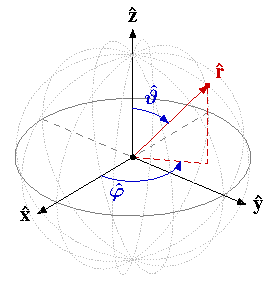
\includegraphics{papers/kugel/figures/tikz/spherical-coordinates}
  \caption{
    Spherical coordinate system. Space is described with the free variables $r
    \in \mathbb{R}_0^+$, $\vartheta \in [0; \pi]$ and $\varphi \in [0; 2\pi)$.
    \label{kugel:fig:spherical-coordinates}
  }
\end{figure}

From Section \ref{buch:pde:section:kugel}, we know that the spherical Laplacian
in the spherical coordinate system (shown in Figure
\ref{kugel:fig:spherical-coordinates}) is is defined as
\begin{equation*}
    \sphlaplacian :=
      \frac{1}{r^2} \frac{\partial}{\partial r} \left(
        r^2 \frac{\partial}{\partial r}
      \right)
      + \frac{1}{r^2} \left[
          \frac{1}{\sin\vartheta} \frac{\partial}{\partial \vartheta} \left(
            \sin\vartheta \frac{\partial}{\partial\vartheta}
          \right)
        + \frac{1}{\sin^2 \vartheta} \frac{\partial^2}{\partial\varphi^2}
      \right].
\end{equation*}
But we will not consider this algebraic monstrosity in its entirety. As the
title suggests, we will only care about the \emph{surface} of the sphere.  This
is for many reasons, but mainly to simplify reduce the already broad scope of
this text. Concretely, we will always work on the unit sphere, which just means
that we set $r = 1$ and keep only $\vartheta$ and $\varphi$ as free variables.
Now, since the variable $r$ became a constant, we can leave out all derivatives
with respect to $r$ and substitute all $r$'s with 1's to obtain a new operator
that deserves its own name.

\begin{definition}[Surface spherical Laplacian]
  \label{kugel:def:surface-laplacian}
  The operator
  \begin{equation*}
      \surflaplacian :=
        \frac{1}{\sin\vartheta} \frac{\partial}{\partial \vartheta} \left(
          \sin\vartheta \frac{\partial}{\partial\vartheta}
        \right)
        + \frac{1}{\sin^2 \vartheta} \frac{\partial^2}{\partial\varphi^2},
  \end{equation*}
  is called the surface spherical Laplacian.
\end{definition}

In the definition, the subscript ``$\partial S$'' was used to emphasize the
fact that we are on the spherical surface, which can be understood as being the
boundary of the sphere. But what does it actually do? To get an intuition,
first of all, notice the fact that $\surflaplacian$ have second derivatives,
which means that this a measure of \emph{curvature}; But curvature of what? To
get an even stronger intuition we will go into geometry, were curvature can be
grasped very well visually. Consider figure \ref{kugel:fig:curvature} where the
curvature is shown using colors. First we have the curvature of a curve in 1D,
then the curvature of a surface (2D), and finally the curvature of a function on
the surface of the unit sphere.

\begin{figure}
  \centering
  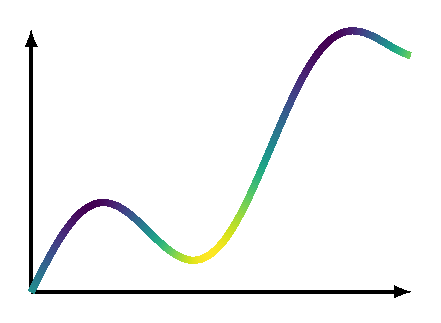
\includegraphics[width=.3\linewidth]{papers/kugel/figures/tikz/curvature-1d}
  \hskip 5mm
  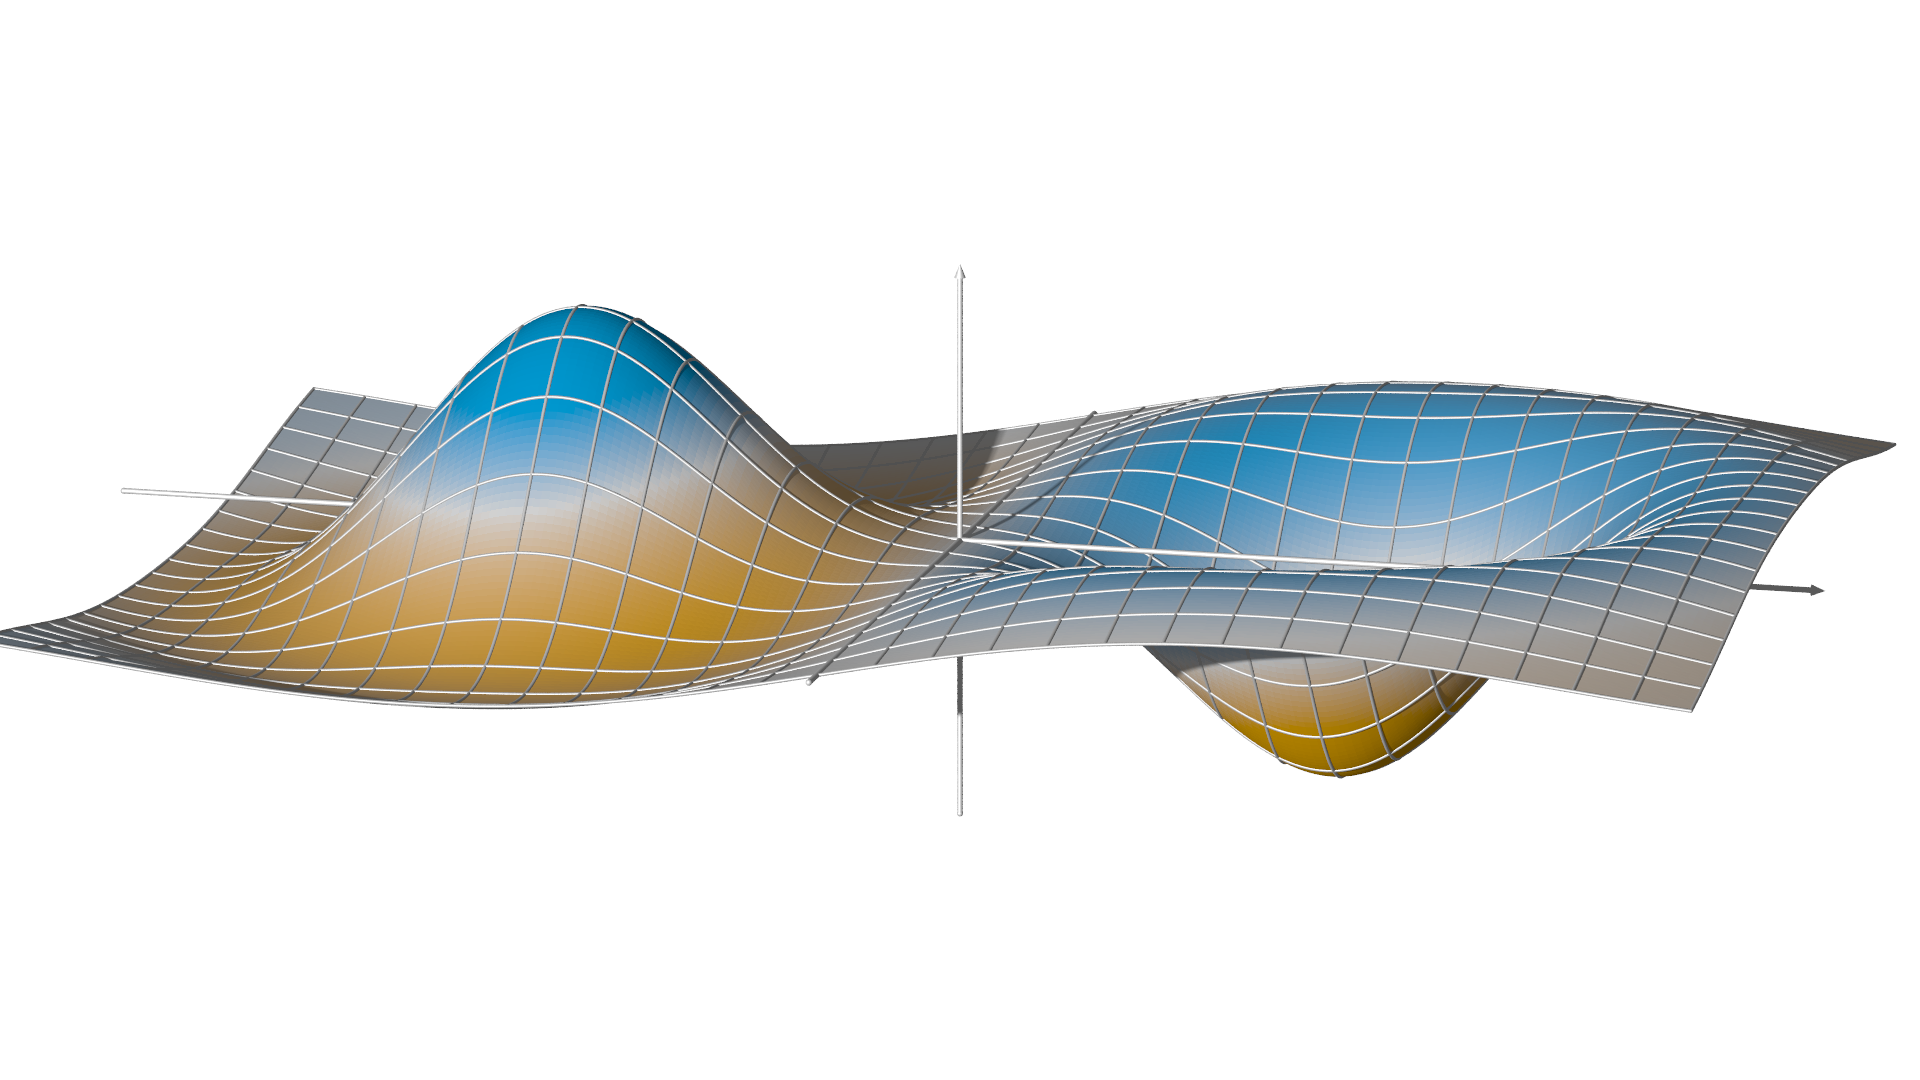
\includegraphics[width=.3\linewidth]{papers/kugel/figures/povray/curvature}
  \hskip 5mm
  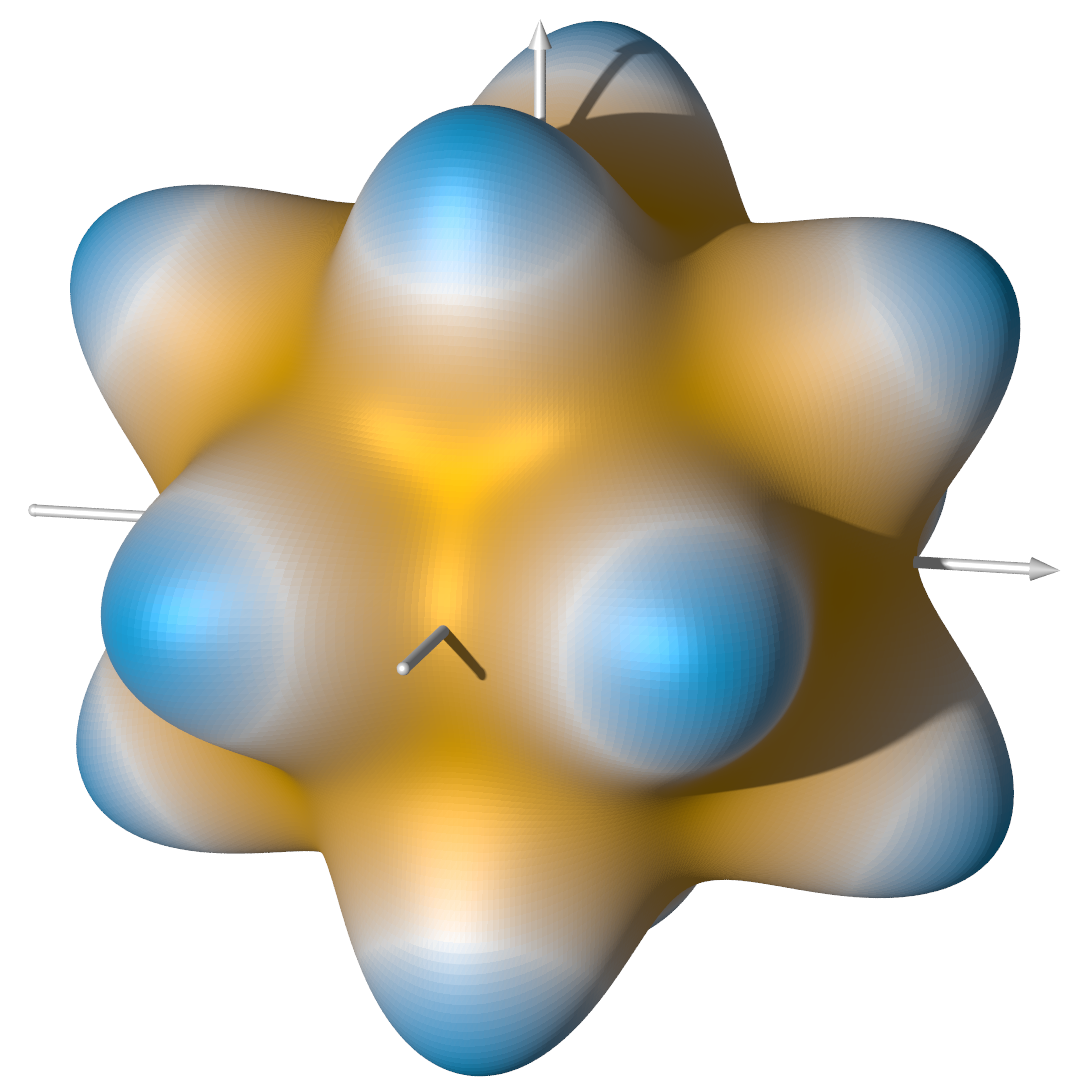
\includegraphics[width=.3\linewidth]{papers/kugel/figures/povray/spherecurve}
  \caption{
    \kugeltodo{Fix alignment / size, add caption. Would be nice to match colors.}
    \label{kugel:fig:curvature}
  }
\end{figure}

Now that we have defined an operator, we can go and study its eigenfunctions,
which means that we would like to find the functions $f(\vartheta, \varphi)$
that satisfy the equation
\begin{equation} \label{kuvel:eqn:eigen}
    \surflaplacian f = -\lambda f.
\end{equation}
Perhaps it may not be obvious at first glance, but we are in fact dealing with a
partial differential equation (PDE). If we unpack the notation of the operator
$\nabla^2_{\partial S}$ according to definition
\ref{kugel:def:surface-laplacian}, we get:
\begin{equation} \label{kugel:eqn:eigen-pde}
    \frac{1}{\sin\vartheta} \frac{\partial}{\partial \vartheta} \left(
      \sin\vartheta \frac{\partial f}{\partial\vartheta}
    \right)
    + \frac{1}{\sin^2 \vartheta} \frac{\partial^2 f}{\partial\varphi^2}
    + \lambda f = 0.
\end{equation}
Since all functions satisfying \eqref{kugel:eqn:eigen-pde} are the
\emph{eigenfunctions} of $\surflaplacian$, our new goal is to solve this PDE.
The task may seem very difficult but we can simplify it with a well-known
technique: \emph{the separation Ansatz}. It consists in assuming that the
function $f(\vartheta, \varphi)$ can be factorized in the following form:
\begin{equation} \label{kugel:eqn:sep-ansatz:0}
    f(\vartheta, \varphi) = \Theta(\vartheta)\Phi(\varphi). 
\end{equation}
In other words, we are saying that the effect of the two independent variables
can be described using the multiplication of two functions that describe their
effect separately. This separation process was already presented in section
\ref{buch:pde:section:kugel}, but we will briefly rehearse it here for
convenience. If we substitute this assumption in
\eqref{kugel:eqn:eigen-pde}, we have:
\begin{equation} \label{kugel:eqn:sep-ansatz:1}
    \frac{1}{\sin\vartheta} \frac{\partial}{\partial \vartheta} \left(
      \sin\vartheta \frac{\partial  \Theta(\vartheta)}{\partial\vartheta}
    \right) \Phi(\varphi)
    + \frac{1}{\sin^2 \vartheta} \frac{\partial^2 \Phi(\varphi)}{\partial\varphi^2}
      \Theta(\vartheta)
    + \lambda \Theta(\vartheta)\Phi(\varphi) = 0.
\end{equation}
Dividing by $\Theta(\vartheta)\Phi(\varphi)$ and introducing an auxiliary
variable $m$, the separation constant, yields:
\begin{equation*}
  \frac{1}{\Theta(\vartheta)}\sin \vartheta \frac{d}{d \vartheta} \left(
    \sin \vartheta \frac{d \Theta}{d \vartheta}
  \right)
  + \lambda \sin^2 \vartheta
  = -\frac{1}{\Phi(\varphi)} \frac{d^2\Phi(\varphi)}{d\varphi^2}
  = m,
\end{equation*}
which is equivalent to the following system of 2 first order differential
equations (ODEs):
\begin{subequations}
  \begin{gather}
    \frac{d^2\Phi(\varphi)}{d\varphi^2} = -m \Phi(\varphi),
      \label{kugel:eqn:ode-phi} \\ 
    \sin \vartheta \frac{d}{d \vartheta} \left(
      \sin \vartheta \frac{d \Theta}{d \vartheta}
    \right)
    + \left( \lambda - \frac{m}{\sin^2 \vartheta} \right)
      \Theta(\vartheta) = 0
      \label{kugel:eqn:ode-theta}.
  \end{gather}
\end{subequations}
The solution of \eqref{kugel:eqn:ode-phi} is easy to find: The complex
exponential is obviously the function we are looking for. So we can directly
write the solutions
\begin{equation} \label{kugel:eqn:ode-phi-sol}
    \Phi(\varphi) = e^{i m \varphi}, \quad m \in \mathbb{Z}.
\end{equation}
The restriction that the separation constant $m$ needs to be an integer arises
from the fact that we require a $2\pi$-periodicity in $\varphi$ since
$\Phi(\varphi + 2\pi) = \Phi(\varphi)$. Unfortunately, solving
\eqref{kugel:eqn:ode-theta} is not so straightforward. Actually it is quite
difficult, and the process is so involved that it will require a dedicated
section of its own.

\subsection{Legendre Functions}

To solve \eqref{kugel:eqn:ode-theta}
We can begin by considering the substitution $x = \cos \vartheta$. The operator $\frac{d}{d \vartheta}$ will be:
\begin{align*}
    \frac{d}{d \vartheta} = \frac{dx}{d \vartheta}\frac{d}{dx} &= -\sin \vartheta \frac{d}{dx} \\
    &= -\sqrt{1-x^2} \frac{d}{dx}.
\end{align*} 
Eq.(\ref{kugel:eq:ODE_2}) will then become.
\begin{align*}
   \frac{-\sqrt{1-x^2}}{\sqrt{1-x^2}} \frac{d}{dx} \left( \left(\sqrt{1-x^2}\right) \left(-\sqrt{1-x^2}\right) \frac{d \Theta}{dx} \right) + \left( \lambda - \frac{m}{\sin^2 \vartheta} \right)\Theta(\vartheta) &= 0 \\
   \frac{d}{dx} \left( (1-x^2) \frac{d \Theta}{dx} \right) + \left( \lambda - \frac{m}{\sin^2 \vartheta} \right)\Theta(\vartheta) &= 0 \\
   (1-x^2)\frac{d^2 \Theta}{dx} - 2x\frac{d \Theta}{dx} + \left( \lambda - \frac{m}{\sin^2 \vartheta} \right)\Theta(\vartheta) &= 0 \\
   (1-x^2)\frac{d^2 \Theta}{dx} - 2x\frac{d \Theta}{dx} + \left( \lambda - \frac{m}{1-x^2} \right)\Theta(\vartheta) &= 0 
\end{align*}
By making two final cosmetic substitutions, namely $\Theta(\vartheta)=\Theta(\cos^{-1}x):=y(x)$ and $\lambda=n(n+1)$, we will be able to define the \emph{Associated Legendre Equation} in its standard and most familiar form
\begin{definition}{Associated Legendre Equation}
    \begin{equation}\label{kugel:eq:associated_leg_eq}
        (1-x^2)\frac{d^2 y}{dx} - 2x\frac{d y}{dx} + \left( n(n+1) - \frac{m}{1-x^2} \right)y(x) = 0. 
    \end{equation}
\end{definition}
Our new goal then became solving Eq.(\ref{kugel:eq:asssociated_leg_eq}). After that we can fit the solution into Eq.(\ref{kugel:eq:sep_ansatz_0}), obtaining $f(\vartheta, \varphi)$, the solution of the eigenvalue problem. \newline
We simplified the problem somewhat but the task still remains very difficult. We can rely on a lemma to continue but first we need to define an additional equation, namely the \emph{Legendre Equation}
\begin{definition}{Legendre equation}\newline
    Setting $m=0$ in Eq.(\ref{kugel:eq:asssociated_leg_eq}), we get
    \begin{equation}\label{kugel:eq:leg_eq}
        (1-x^2)\frac{d^2 y}{dx} - 2x\frac{d y}{dx} + n(n+1)y(x) = 0,
    \end{equation}
    also known as \emph{Legendre Equation}.
\end{definition}
Now we can continue with the lemma
\begin{lemma}\label{kugel:lemma_1}
    If $y_n(x)$ is a solution of Eq.(\ref{kugel:eq:leg_eq}), then the function
    \begin{equation*}
        y_{m,n}(x) = (1-x^2)^{\frac{m}{2}}\frac{d^m}{dx^m}y_n(x)
    \end{equation*}
    satisfies Eq.(\ref{kugel:eq:associated_leg_eq})
\end{lemma}
\begin{proof} [TODO: modificare la $m$ (è già usata come costante di separazione) o forse è giusta (?)]
    To begin, we can start by differentiating $m$ times Eq.\eqref{kugel:eq:leg_eq} (which is staisfied by $y(x)$), obtaining
    \begin{equation}\label{eq:lagrange_mderiv}
    \frac{d^m}{dx^m}\left[ (1-x^2)\frac{d^2y}{dx^2} \right] -2 \frac{d^m}{dx^m}\left[ x\frac{dy}{dx} \right] + n(n+1)\frac{d^m}{dx^m}y=0.
    \end{equation}
    \emph{Leibniz's theorem} says, that if we want to differentiate $m$ times a multiplication of two functions, we can use the binomial coefficients to build up a sum. This allows us to be more compact, obtaining 
    \begin{equation}\label{eq:leibniz}
    \frac{d^m}{dx^m}[u(x)v(x)] = \sum_{i=0}^m \binom{n}{i} \frac{d^{m-i}u}{dx^{m-1}} \frac{d^{i}v}{dx^i}.
    \end{equation}
    Using Eq.\eqref{eq:leibniz} in Eq.\eqref{eq:lagrange_mderiv}, we have
    \begin{align}
    (1-x^2)\frac{d^{m+2}y}{dx^{m+2}} &+ m \frac{d}{dx}(1-x^2)\frac{d^{m+1}y}{dx^{m+1}} + \frac{m(m-1)}{2}\frac{d^{2}}{dx^{2}}(1-x^2)\frac{d^{m}y}{dx^{m}} + n(n+1)\frac{d^m{}y}{dx^{m}} \nonumber \\
    &-2\left(x\frac{d^{m+1}y}{dx^{m+1}} + m\frac{d}{dx}x\frac{d^{m}y}{dx^{m}} \right) \nonumber \\
    &= (1-x^2)\frac{d^{m+2}y}{dx^{m+2}} -2x(m+1)\frac{d^{m+1}y}{dx^{m+1}}+(n(n+1)-m(m-1)-2m)\frac{d^{m}y}{dx^{m}}=0. \label{eq:aux_3}
    \end{align}
    To make the notation easier to follow, a new function can be defined
    \begin{equation*}
    \frac{d^{m}y}{dx^{m}} := y_m.
    \end{equation*}
    Eq.\eqref{eq:aux_3} now becomes
    \begin{equation}\label{eq:1st_subs}
    (1-x^2)\frac{d^{2}y_m}{dx^{2}} -2x(m+1)\frac{dy_m}{dx}+(n(n+1)-m(m+1))y_m=0
    \end{equation}
    A second function can be further defined as
    \begin{equation*}
    (1-x^2)^{\frac{m}{2}}\frac{d^{m}y}{dx^{m}} = (1-x^2)^{\frac{m}{2}}y_m := \hat{y}_m,
    \end{equation*}
    allowing to write Eq.\eqref{eq:1st_subs} as
    \begin{equation}\label{eq:2st_subs}
    (1-x^2)\frac{d^2}{dx^2}[\hat{y}_m(1-x^2)^{-\frac{m}{2}}] -2(m+1)x\frac{d}{dx}[\hat{y}_m(1-x^2)^{-\frac{m}{2}}] + (n(n+1)-m(m+1))\hat{y}_m(1-x^2)^{-\frac{m}{2}}=0.
    \end{equation}
    The goal now is to compute the two terms 
    \begin{align*}
    \frac{d^2}{dx^2}[\hat{y}_m(1-x^2)^{-\frac{m}{2}}] &=  \frac{d^2\hat{y}_m}{dx^2} (1-x^2)^{-\frac{m}{2}} + \frac{d\hat{y}_m}{dx}\frac{m}{2}(1-x^2)^{-\frac{m}{2}-1}2x \\
    &+ m\left( \frac{d\hat{y}_m}{dx} x (1-x^2)^{-\frac{m}{2}-1} + \hat{y}_m (1-x^2)^{-\frac{m}{2}-1} - \hat{y}_m x (-\frac{m}{2}-1)(1-x^2)^{-\frac{m}{2}} 2x\right) \\
    &= \frac{d^2\hat{y}_m}{dx^2} (1-x^2)^{-\frac{m}{2}} + \frac{d\hat{y}_m}{dx}mx (1-x^2)^{-\frac{m}{2}-1} + m\frac{d\hat{y}_m}{dx}x (1-x^2)^{-\frac{m}{2}-1}\\
    &+ m\hat{y}_m  (1-x^2)^{-\frac{m}{2}-1} + m\hat{y}_m x^2(m+2)(1-x^2)^{-\frac{m}{2}-2}
    \end{align*}
    and
    \begin{align*}
    \frac{d}{dx}[\hat{y}_m(1-x^2)^{-\frac{m}{2}}] &= \frac{d\hat{y}_m}{dx}(1-x^2)^{-\frac{m}{2}} + \hat{y}_m\frac{m}{2}(1-x^2)^{-\frac{m}{2}-1}2x \\
    &= \frac{d\hat{y}_m}{dx}(1-x^2)^{-\frac{m}{2}} + \hat{y}_mm(1-x^2)^{-\frac{m}{2}-1}x,
    \end{align*}
    to use them in Eq.\eqref{eq:2st_subs}, obtaining
    \begin{align*}
    (1-x^2)\biggl[\frac{d^2\hat{y}_m}{dx^2} (1-x^2)^{-\frac{m}{2}} &+ \frac{d\hat{y}_m}{dx}mx (1-x^2)^{-\frac{m}{2}-1} + m\frac{d\hat{y}_m}{dx}x (1-x^2)^{-\frac{m}{2}-1} \\ 
    &+ m\hat{y}_m  (1-x^2)^{-\frac{m}{2}-1} + m\hat{y}_m x^2(m+2)(1-x^2)^{-\frac{m}{2}-2}\biggr] \\
    &-2(m+1)x\left[  \frac{d\hat{y}_m}{dx}(1-x^2)^{-\frac{m}{2}} + \hat{y}_mm(1-x^2)^{-\frac{m}{2}-1}x \right] \\
    &+ (n(n+1)-m(m+1))\hat{y}_m(1-x^2)^{-\frac{m}{2}}=0.\\
    \end{align*}
    We can now divide by $(1-x^2)^{-\frac{m}{2}}$, obtaining
    \begin{align*}
    (1-x^2)\biggl[\frac{d^2\hat{y}_m}{dx^2} &+ \frac{d\hat{y}_m}{dx}mx (1-x^2)^{-1} + m\frac{d\hat{y}_m}{dx}x (1-x^2)^{-1} + m\hat{y}_m  (1-x^2)^{-1} + m\hat{y}_m x^2(m+2)(1-x^2)^{-2}\biggr] \\
    &-2(m+1)x\left[  \frac{d\hat{y}_m}{dx} + \hat{y}_mm(1-x^2)^{-1}x \right] + (n(n+1)-m(m+1))\hat{y}_m\\
    &= \frac{d^2\hat{y}_m}{dx^2} + \frac{d\hat{y}_m}{dx}mx + m\frac{d\hat{y}_m}{dx}x + m\hat{y}_m + m\hat{y}_m x^2(m+2)(1-x^2)^{-1} \\
    &-2(m+1)x\left[  \frac{d\hat{y}_m}{dx} + \hat{y}_mm(1-x^2)^{-1}x \right] + (n(n+1)-m(m+1))\hat{y}_m\\
    \end{align*}
    and collecting some terms
    \begin{equation*}
    (1-x^2)\frac{d^2\hat{y}_m}{dx^2} - 2x\frac{d\hat{y}_m}{dx} + \left( -x^2 \frac{m^2}{1-x^2} + m+n(n+1)-m(m+1)\right)\hat{y}_m=0.
    \end{equation*}
    Showing that 
    \begin{align*}
    -x^2 \frac{m^2}{1-x^2} + m+n(n+1)-m(m+1) &= n(n+1)- m^2 -x^2 \frac{m^2}{1-x^2} \\
    &= n(n+1)- \frac{m}{1-x^2}
    \end{align*}
    implies $\hat{y}_m(x)$ being a solution of Eq.\eqref{kugel:eq:associated_leg_eq}
\end{proof}
In simpler words, if we find a solution to Eq.\eqref{kugel:eq:leg_eq}, we can extend the latter according to the Lemma \ref{kugel:lemma_1} obtaining the solution of Eq.\eqref{kugel:eq:associated_leg_eq}.\newline
We can say that we are going in the right direction, as the problem to be solved is decreasing in difficulty. We moved from having to find a solution to Eq.\eqref{kugel:eq:associated_leg_eq} to finding a solution to Eq.\eqref{kugel:eq:leg_eq}, which is much more approachable as a problem. Luckily for us, the lemma we will present below will help us extensively, which is something of an euphemism, since it will give us the solution directly.
\begin{lemma}
    The polynomial function
    \begin{align*}
        y_n(x)&=\sum_{k=0}^{\lfloor \frac{n}{2} \rfloor} (-1)^k \frac{(2n-2k)!}{2^n k! (n-k)!(n-2k)!} x^{n-2k}\\
        &= \frac{1}{n!2^n}\frac{d^n}{dx^n}(1-x^2)^n =: P_n(x),
    \end{align*}
    is a solution to the second order differential equation
    \begin{equation}\label{kugel:eq:sol_leg}
        (1-x^2)\frac{d^2y}{dx^2}-2x\frac{dy}{dx} + n(n+1)y=0, \quad \forall n>0.
    \end{equation}
\end{lemma}
\begin{proof}
    In order to find a solution to Eq.\eqref{eq:legendre}, the following Ansatz can be performed:
    \begin{equation}\label{eq:ansatz}
    y(x) = \sum_{k=0}^\infty a_k x^k.
    \end{equation}
    Given Eq.\eqref{eq:ansatz}, then
    \begin{align*}
    \frac{dy}{dx} &= \sum_{k=0}^\infty k a_k x^{k-1}, \\
    \frac{d^2y}{dx^2} &= \sum_{k=0}^\infty k (k-1) a_k x^{k-2}.
    \end{align*}
    Eq.\eqref{eq:legendre} can be therefore written as
    \begin{align}
    &(1-x^2)\sum_{k=0}^\infty k (k-1) a_k x^{k-2} - 2x\sum_{k=0}^\infty k a_k x^{k-1} + n(n+1)\sum_{k=0}^\infty a_k x^k=0 \label{eq:ansatz_in_legendre} \\
    &=\sum_{k=0}^\infty k (k-1) a_k x^{k-2} - \sum_{k=0}^\infty k (k-1) a_k x^{k} - 2x\sum_{k=0}^\infty k a_k x^{k-1} + n(n+1)\sum_{k=0}^\infty a_k x^k=0. \nonumber
    \end{align}
    If one consider the term
    \begin{equation}\label{eq:term}
    \sum_{k=0}^\infty k (k-1) a_k x^{k-2},
    \end{equation}
    the substitution $\tilde{k}=k-2$ yields Eq.\eqref{eq:term} to
    \begin{equation*}
    \sum_{\tilde{k}=-2}^\infty (\tilde{k}+2) (\tilde{k}+1) a_{\tilde{k}+2} x^{\tilde{k}}=\sum_{\tilde{k}=0}^\infty (\tilde{k}+2) (\tilde{k}+1) a_{\tilde{k}} x^{\tilde{k}}.
    \end{equation*}
    This means that Eq.\eqref{eq:ansatz_in_legendre} becomes
    \begin{align}
    &\sum_{k=0}^\infty (k+1)(k+2) a_{k+2} x^{k} - \sum_{k=0}^\infty k (k-1) a_k x^{k} - 2\sum_{k=0}^\infty k a_k x^k + n(n+1)\sum_{k=0}^\infty a_k x^k \nonumber \\
    = &\sum_{k=0}^\infty \big[ (k+1)(k+2) a_{k+2} - k (k-1) a_k - 2 k a_k + n(n+1) a_k \big] x^k \stackrel{!}{=} 0. \label{eq:condition}
    \end{align}
    The condition in Eq.\eqref{eq:condition} is equivalent to 
    \begin{equation}\label{eq:condition_2}
    (k+1)(k+2) a_{k+2} - k (k-1) a_k - 2 k a_k + n(n+1) a_k = 0.
    \end{equation}
    We can derive a recursion formula for $a_{k+2}$ from Eq.\eqref{eq:condition_2}, which can be expressed as
    \begin{equation}\label{eq:recursion}
    a_{k+2}= \frac{k (k-1) - 2 k + n(n+1)}{(k+1)(k+2)}a_k = \frac{(k-n)(k+n+1)}{(k+2)(k+1)}a_k.
    \end{equation}
    All coefficients can be calculated using the latter. 
    
    Following Eq.\eqref{eq:recursion}, if we want to compute $a_6$ we would have
    \begin{align*}
    a_{6}= -\frac{(n-4)(n+5)}{6\cdot 5}a_4 &= -\frac{(n-4)(5+n)}{6 \cdot 5} -\frac{(n-2)(n+3)}{4 \cdot 3}  a_2 \\
    &= -\frac{(n-4)(n+5)}{6 \cdot 5} -\frac{(n-2)(n+3)}{4 \cdot 3} -\frac{n(n+1)}{2 \cdot 1}  a_0 \\
    &= -\frac{(n+5)(n+3)(n+1)n(n-2)(n-4)}{6!} a_0.
    \end{align*}
    One can generalize this relation for the $i^\text{th}$ even coefficient as
    \begin{equation*}
    a_{2k} = (-1)^k \frac{(n+(2k-1))(n+(2k-1)-2)\hdots (n-(2k-2)+2)(n-(2k-2))}{(2k)!}a_0
    \end{equation*}
    where $i=2k$.
    
    A similar expression can be written for the odd coefficients $a_{2k-1}$. In this case, the equation starts from $a_1$ and to find the pattern we can write the recursion for an odd coefficient, $a_7$ for example
    \begin{align*}
    a_{7}= -\frac{(n-5)(n+6)}{7\cdot 6}a_5 &= - \frac{(n-5)(n+6)}{7\cdot 6} -\frac{(n-3)(n+4)}{5 \cdot 4}  a_3 \\
    &= - \frac{(n-5)(n+6)}{7\cdot 6} -\frac{(n-3)(n+4)}{5 \cdot 4}  -\frac{(n-1)(n+2)}{3 \cdot 2}  a_1 \\
    &= -\frac{(n+6)(n+4)(n+2)(n-1)(n-3)(n-5)}{7!} a_1.
    \end{align*}
    As before, we can generalize this equation for the $i^\text{th}$ odd coefficient
    \begin{equation*}
    a_{2k+1} = (-1)^k \frac{(n + 2k)(n+2k-2)\hdots(n-(2k-1)+2)(n-(2k-1))}{(2k+1)!}a_1
    \end{equation*}
    where $i=2k+1$.
    
    Let be 
    \begin{align*}
    y_\text{e}^K(x) &:= \sum_{k=0}^K(-1)^k \frac{(n+(2k-1))(n+(2k-1)-2)\hdots \color{red}(n-(2k-2)+2)(n-(2k-2))}{(2k)!} x^{2k}, \\
    y_\text{o}^K(x) &:= \sum_{k=0}^K(-1)^k \frac{(n + 2k)(n+2k-2)\hdots \color{blue} (n-(2k-1)+2)(n-(2k-1))}{(2k+1)!} x^{2k+1}.
    \end{align*}
    The solution to the Eq.\eqref{eq:legendre} can be written as
    \begin{equation}\label{eq:solution}
    y(x) = \lim_{K \to \infty} \left[ a_0 y_\text{e}^K(x) + a_1 y_\text{o}^K(x) \right].
    \end{equation}
    
    The colored parts can be analyzed separately:
    \begin{itemize}
      \item[\textcolor{red}{\textbullet}] Suppose that $n=n_0$ is an even number. Then the red part, for a specific value of $k=k_0$, will follow the following relation:
    \begin{equation*}
    n_0-(2k_0-2)=0. 
    \end{equation*}
    From that point on, given the recursive nature of Eq.\eqref{eq:recursion}, all the subsequent coefficients will also be 0, making the sum finite.
    \begin{equation*}
    a_{2k}=0 \iff y_{\text{o}}^{2k}(x)=y_{\text{o}}^{2k_0}(x), \quad \forall k>k_0
    \end{equation*} 
      \item[\textcolor{blue}{\textbullet}] Suppose that $n=n_0$ is an odd number. Then the blue part, for a specific value of $k=k_0$, will follow the following relation 
    \begin{equation*}
    n_0-(2k_0-1)=0.  
    \end{equation*}
    From that point on, for the same reason as before, all the subsequent coefficients will also be 0, making the sum finite.
    \begin{equation*}
    a_{2k+1}=0 \iff y_{\text{o}}^{2k+1}(x)=y_{\text{o}}^{2k_0+1}(x), \quad \forall k>k_0
    \end{equation*}
    \end{itemize} 
    
    There is the possibility of expressing the solution in Eq.\eqref{eq:solution} in a more compact form, combining the two solutions $y_\text{o}^K(x)$ and $y_\text{e}^K(x)$. They are both a polynomial of maximum degree $n$, assuming $n \in \mathbb{N}$. In the case where $n$ is even, the polynomial solution
    \begin{equation*}
    \lim_{K\to \infty} y_\text{e}^K(x)
    \end{equation*}
    will be a finite sum. If instead $n$ is odd, will be 
    \begin{equation*}
    \lim_{K\to \infty} y_\text{o}^K(x)
    \end{equation*}
    to be a finite sum. 
    
    Depending on the coefficient we start with, $a_1$ or $a_0$, we will obtain the odd or even polynomial respectively. Starting with the last coefficient $a_n$ and, recursively, calculating all the others in descending order, we can express the two parts $y_\text{o}^K(x)$ and $y_\text{e}^K(x)$ with a single sum. Hence, because we start with the last coefficient, the choice concerning $a_1$ and $a_0$ will be at the end of the sum, and not at the beginning. To compact Eq.\eqref{eq:solution}, Eq.\eqref{eq:recursion} can be reconsidered to calculate the coefficient $a_{k-2}$, using $a_k$
    \begin{equation*}
    a_{k-2} = -\frac{(k+2)(k+1)}{(k-n)(k+n+1)}a_k
    \end{equation*}
    Now the game is to find a pattern, as before. Remember that $n$ is a fixed parameter of Eq.\eqref{eq:legendre}.  
    \begin{align*}
    a_{n-2} &= -\frac{n(n-1)}{2(2n-1)}a_n, \\
    a_{n-4} &= -\frac{(n-2)(n-3)}{4(2n-3)}a_{n-2} \\
    &= -\frac{(n-2)(n-3)}{4(2n-3)}-\frac{n(n-1)}{2(2n-1)}a_n.
    \end{align*}
    In general 
    \begin{equation}\label{eq:general_recursion}
    a_{n-2k} = (-1)^k \frac{n(n-1)(n-2)(n-3) \hdots (n-2k+1)}{2\cdot4\hdots 2k(2n-1)(2n-3)\hdots(2n-2k+1)}a_n
    \end{equation}
    The whole solution can now be written as
    \begin{align}
    y(x) &= a_n x^n + a_{n-2} x^{n-2} + a_{n-4} x^{n-4} + a_{n-6} x^{n-6} + \hdots + \begin{cases} 
    a_1 x, \quad &\text{if } n \text{ odd} \\ 
    a_0, \quad  &\text{if } n \text{ even} 
    \end{cases} \nonumber \\
    &= \sum_{k=0}^{\lfloor \frac{n}{2} \rfloor} a_{n-2k}x^{n-2k} \label{eq:solution_2}
    \end{align}
    By considering
    \begin{align}
    (2n-1)(2n-3)\hdots (2n-2k+1)&=\frac{2n(2n-1)(2n-2)(2n-3)\hdots(2n-2k+1)}
    {2n(2n-2)(2n-4)(2n-6)\hdots(2n-2k+2)} \nonumber \\ 
    &=\frac{\frac{(2n)!}{(2n-2k)!}}
    {2^kn(n-1)(n-2)(n-3)\hdots(n-k+1)} \nonumber \\
    &=\frac{\frac{(2n)!}{(2n-2k)!}}
    {2^k\frac{n!}{(n-k)!}}=\frac{(n-k)!(2n)!}{n!(2n-2k)!2^k} \label{eq:1_sub_recursion}, \\
    2 \cdot 4  \hdots 2k &= 2^r 1\cdot2 \hdots r = 2^r r!\label{eq:2_sub_recursion}, \\
    n(n-1)(n-2)(n-3) \hdots (n-2k+1) &= \frac{n!}{(n-2k)!}\label{eq:3_sub_recursion}.
    \end{align}
    Eq.\eqref{eq:solution_2} can be rewritten as
    \begin{equation}\label{eq:solution_3}
    y(x)=a_n \sum_{k=0}^{\lfloor \frac{n}{2} \rfloor} (-1)^k \frac{n!^2(2n-2k)!}{k!(n-2k)!(n-k)!(2n)!}  x^{n-2k}.
    \end{equation}
    Eq.\eqref{eq:solution_3} is defined for any $a_n$. By letting $a_n$ be declared as
    \begin{equation*}
    a_{n} := \frac{(2n)!}{2^n n!^2},
    \end{equation*}
    the so called \emph{Legendre polynomial} emerges
    \begin{equation}\label{eq:leg_poly}
    P_n(x):=\sum_{k=0}^{\lfloor \frac{n}{2} \rfloor} (-1)^k \frac{(2n-2k)!}{2^n k! (n-k)!(n-2k)!} x^{n-2k} 
    \end{equation}
\end{proof}
As can be seen, the solution is a $n$-dependent power series, traditionally denoted as $P_n(x)$. This set of polynomials are called \emph{Legendre Polynomials}, because precisely they are polynomials satisfying the Legendre equation.\newline
Now that we have a solution to Eq.\eqref{kugel:eq:leg_eq}, we can then extend Eq.\eqref{kugel:eq:sol_leg}, as stated in Lemma \ref{kugel:lemma_1}. We will then have
\begin{align*}
y_{m,n}(x) &= (1-x^2)^{\frac{m}{2}}\frac{d^m}{dx^m}P_n(x) \\
&= \frac{1}{n!2^n}(1-x^2)^{\frac{m}{2}}\frac{d^{m+n}}{dx^{m+n}}(1-x^2)^n 
\end{align*}
This set of functions are defined as \emph{Associated Legendre functions}, because similarly to before, they solve the Associated Legendre equation, defined in Eq.\eqref{kugel:eq:eq_leg}.
\begin{definition}{Associated Legendre Functions}
\begin{equation}\label{kugel:eq:associated_leg_func}
P_{m,n}(x) := \frac{1}{n!2^n}(1-x^2)^{\frac{m}{2}}\frac{d^{m+n}}{dx^{m+n}}(1-x^2)^n 
\end{equation}
\end{definition}
As you may recall, previously we performed the substitution $x=\cos \vartheta$. Now we need to return to the old domain, which can be done straightforwardly:
\begin{equation*}
    \Theta(\vartheta) = P_{m,n}(\cos \vartheta),
\end{equation*}
obtaining the much sought function $\Theta(\vartheta)$. \newline
So we finally reached the end of this tortuous path. Now we just need to put together all the information we have to construct $f(\vartheta, \varphi)$ in the following way:
\begin{equation}\label{kugel:eq:sph_harm_0}
    f(\vartheta, \varphi) = \Theta(\vartheta)\Phi(\varphi) = P_{m,n}(\cos \vartheta)e^{jm\varphi}, \quad |m|\leq n.
\end{equation}
The constraint $|m|<n$, can be justified by considering Eq.\eqref{kugel:eq:associated_leg_func}, in which the derivative of degree $m+n$ is present. A derivative to be well defined must have an order that is greater than zero. Furthermore, it can be seen that this derivative is applied on a polynomial of degree $2n$. As is known from Calculus 1, if you derive a polynomial of degree $2n$ more than $2n$ times, you get zero, which is a trivial solution in which we are not interested.\newline
We can thus summarize these two conditions by writing:
\begin{equation*}
    \begin{rcases}
        m+n \leq 2n &\implies m \leq n \\
        m+n \geq 0  &\implies  m \geq -n
    \end{rcases} |m| \leq n.
\end{equation*}
The set of functions in Eq.\eqref{kugel:eq:sph_harm_0} is named \emph{Spherical Harmonics}, which are the eigenfunctions of the Laplace operator on the \emph{spherical surface domain}, which is exactly what we were looking for at the beginning of this section.
\begin{definition}{Spherical Harmonics}
    \begin{equation}\label{kugel:eq:sph_harm_1}
    \tilde{Y}_{m,n}(\vartheta, \varphi) := P_{m,n}(\cos \vartheta)e^{jm\varphi}, \quad |m|\leq n.
    \end{equation}
\end{definition}

\subsection{Normalization}
As explained in the chapter \ref{}, the concept of orthogonality is very important and at the practical level it is very useful, because it allows us to develop very powerful techniques at the mathematical level.\newline 
Throughout this book we have been confronted with the Sturm-Liouville theory (see chapter \ref{}). The latter, among other things, carries with it the concept of orthogonality. Indeed, if we consider the solutions of the Sturm-Liouville equation, which can be expressed in this form
\begin{equation}\label{kugel:eq:sturm_liouville}
    \mathcal{S}f := \frac{d}{dx}\left[p(x)\frac{df}{dx}\right]+q(x)f(x)
\end{equation}
possiamo dire che formano una base ortogonale.\newline
Adesso possiamo dare un occhiata alle due equazioni che abbiamo ottenuto tramite la Separation Ansatz (Eqs.\eqref{kugel:eq:associated_leg_eq}\eqref{kugel:eq:ODE_1}), le quali possono essere riscritte come:
\begin{align*}
    \frac{d}{dx} \left[ (1-x^2) \cdot \frac{dP_{m,n}}{dx} \right] &+ \left(n(n+1)-\frac{m}{1-x^2} \right) \cdot P_{m,n}(x) = 0, \\
    \frac{d}{d\varphi} \left[ 1 \cdot \frac{ d\Phi }{d\varphi} \right] &+ 1 \cdot \Phi(\varphi) = 0. 
\end{align*}
Si può concludere in modo diretto che sono due casi dell'equazione di Sturm-Liouville. Questo significa che le loro soluzioni sono ortogonali sotto l'inner product con weight function $w(x)=1$, dunque:
\begin{align}
\int_{0}^{2\pi} \Phi_m(\varphi)\Phi_m'(\varphi) d\varphi &= \delta_{m'm}, \nonumber \\
\int_{-1}^1 P_{m,m'}(x)P_{n,n'}(x) dx &= \delta_{m'm}\delta_{n'n}. \label{kugel:eq:orthogonality_associated_func}
\end{align}
Inoltre, possiamo provare l'ortogonalità di $\Theta(\vartheta)$ utilizzando \eqref{kugel:eq:orthogonality_associated_func}:
\begin{align}
    x
\end{align}
Ora, visto che la soluzione dell'eigenfunction problem è formata dalla moltiplicazione di $\Phi_m(\varphi)$ e $P_{m,n}(x)$
\begin{lemma}

\end{lemma}
\subsection{Properties}

\subsection{Recurrence Relations}

\section{Series Expansions in \(C(S^2)\)}

\nocite{olver_introduction_2013}
